% !TeX root = ../note.tex
\section{Используемые инструменты и технологии}\label{sec:tools}

Выбор технологий является важным предварительным этапом разработки сложных информационных систем. Платформа и язык программирования, на котором будет реализована система, заслуживает большого внимания, так как исследования показали, что выбор языка программирования влияет на производительность труда программистов и качество создаваемого ими кода~\cite{code_complete}. % page 59

Ниже перечислены некоторые факторы, повлиявшие на выбор технологий:
\begin{enumerate}
    \item Разрабатываемое ПО должно работать как на операционной системе Windows, так и на популярных дистрибутивах Linux — серверной Ubuntu 18.10 и серверной Ubuntu 20.10.
    \item ПО требовательно к скорости работы технологий. По этой причине, такие языки как Python или Java не могут быть использованы.
    \item Используемый язык должен предоставлять широкие набор наборы библиотек, которые позволят сократить затраты на разработку непрофильных вещи для проекта, такие как логирование, низкоуровневая работа базами данных и т.п.
    \item Код проекта может дорабатываться другими разработчиками.
\end{enumerate}

\subsection{\csharp}

Исходя из вышеперечисленных факторов можно рассмотреть лишь некоторые популярные языки программирования, у которых обширная база библиотек, готовых для использования, а также поддерживается платформа Windows и Linux. Таким образом круг выбора сужается до следующих языков:
\begin{itemize}
    \item C++;
    \item Rust;
    \item \csharp.
\end{itemize}

Язык программирования С++ — компилируемый, статически типизированный язык программирования общего назначения. Поддерживает такие парадигмы программирования, как процедурное программирование, объектно-ориентированное программирование, обобщённое программирование. Язык имеет богатую стандартную библиотеку, которая включает в себя распространённые контейнеры и алгоритмы, ввод-вывод, регулярные выражения, поддержку многопоточности и другие возможности. C++ сочетает свойства как высокоуровневых, так и низкоуровневых языков. В сравнении с его предшественником — языком C, — наибольшее внимание уделено поддержке объектно-ориентированного и обобщённого программирования.

C++ широко используется для разработки программного обеспечения, являясь одним из самых популярных языков программирования. Область его применения включает создание операционных систем, разнообразных прикладных программ, драйверов устройств, приложений для встраиваемых систем, высокопроизводительных серверов, а также игр.

У языка C++ существует ряд проблем, вызванных историческим желанием сохранения совместимости с языком C. Синтаксис языка может вызывать проблемы в силу своей сложности, а разработчики всё реже выбирают C++ своим основным языком программирования. Поэтому C++ будет сложно поддерживать другим разработчикам. Также, несмотря на то, что у языка есть обширные библиотеки, не существует единого стандарта для их установки, поэтому у проекта с множеством зависимостей могут быть проблемы со сборкой, линковкой и несовместимостью различных библиотек.


Рассмотрим следующий вариант — язык Rust. Rust — современный мультипарадигмальный компилируемый язык программирования общего назначения. Разработка языка ведётся сообществом Mozilla Research и финансируется из фонда Mozilla Foundation. Сочетает парадигмы функционального и процедурного программирования с объектной системой, основанной на типажах. Управление памятью осуществляется через механизм ''владения`` с использованием аффинных типов, что позволяет обходиться без системы сборки мусора во время исполнения программы. Объектно-ориентированное программирование поддерживается при помощи отличных от многих языков абстракций.

Ключевые отличия языка: безопасность, скорость и параллелизм. Rust пригоден для системного программирования, в частности, используется для разработки ядер операционных систем. Rust сопоставим по скорости и возможностям с C++/Си, однако гарантирует безопасную работу с памятью, что является встроенным свойством архитектуры языка. Производительность программ на Rust обеспечивается за счёт использования ''абстракций с нулевой стоимостью``.

Rust достаточно молодой язык. Он обладает своей системой сборки и менеджером пакетов, но к сожалению на данный момент экосистема языка ещё слабо развита. Rust пока сложен в поддержке в силу своей нераспространённости, а также из-за использования нетривиальной объектной системы.


Следующий вариант — \csharp. \csharp — объектно-ориентированный язык программирования. Разработан в 1998—2001 годах группой инженеров компании Microsoft под руководством Андерса Хейлсберга и Скотта Вильтаумота как язык разработки приложений для платформы Microsoft .NET Framework. Впоследствии был стандартизирован как ECMA-334 и ISO/IEC 23270~\cite{wiki_dodiez}.

\csharp относится к семье языков с C-подобным синтаксисом, из них его синтаксис наиболее близок к C++ и Java. Язык имеет статическую типизацию, поддерживает полиморфизм, перегрузку операторов (в том числе операторов явного и неявного приведения типа), делегаты, атрибуты, события, свойства, обобщённые типы и методы, итераторы, анонимные функции с поддержкой замыканий, LINQ, исключения, комментарии в формате XML.

Далее рассмотрим некоторые особенности и полезные пакеты \csharp.

\bigskip
\textbf{Пакеты}

Программа на \csharp может быть написана с нуля без использования каких-либо пакетов. Однако платформа .NET предлагает удобную систему управления пакетов NuGet. Она ответственна за копирование файлов библиотеки и автоматическое обновление проекта при выходе новых версий~\cite{wiki_nuget}. Это позволяет .NET программистам значительно увеличить скорость разработки приложений за счёт использования готовых решений.

\bigskip
\textbf{Обработка ошибок и исключительных ситуаций}

Язык \csharp поддерживает стандартный синтаксис обработки исключений характерный для большинства современных языков программирования и предполагающий генерацию исключений специальной командой throw (в некоторых языках raise) и их обработку в блоке try-catch.

\bigskip
\textbf{Кроссплатформенность}

Благодаря платформе .NET (ранее известна как .NET Core) приложения написанные на \csharp могут быть запущены на любой поддерживаемой платформе, включая Windows, Linux и MacOS. Специфические для платформы зависимости будут автоматически загружены при сборке приложения, что значительное увеличивает гибкость разработки.

\bigskip
\textbf{Entity Framework Core}

Entity Framework Core – технология доступа к базам данных от Microsoft. Она позволяет взаимодействовать с СУБД при помощи класов и объектов .NET, а не таблиц конкретной базы данных~\cite{enity_framework}.

В процессе разработки вполне вероятна ситуация, что класс модели изменился, и приходится удалять и базу данных, чтобы сохранялось соответствие модели. Но при удалении базы данных удаляются и все данные из нее. Entity Framework Core предоставляет функционал миграций, который позволяет последовательно применять изменения схемы к базе данных, чтобы синхронизировать её с моделью.


\subsection{RabbitMQ}

Для разработки системы надёжного обмена данными между сервисами необходимо использовать какую-либо прослойку, умеющую работать между процессами и гарантирующую доставку данных. Для таких целей подойдёт технология ``очереди сообщений''.

Очередь сообщений — программно-инженерный компонент, используемый для межпроцессного или межпотокового взаимодействия внутри одного процесса. Для обмена сообщениями используется очередь.

Очереди сообщений предоставляют асинхронный протокол передачи данных, означая, что отправитель и получатель сообщения не обязаны взаимодействовать с очередью сообщений одновременно. Размещённые в очереди сообщения хранятся до тех пор, пока получатель не получит их.

В реализациях очереди сообщений с открытым исходным кодом используются три стандарта:

\begin{itemize}
    \item Advanced Message Queuing Protocol (AMQP) — многофункциональный протокол очереди сообщений;
    \item STOMP  — простой текстовый протокол сообщений;
    \item MQTT — протокол облегчённой очереди сообщений, особенно для встроенных устройств.
\end{itemize}

В данном дипломном проекте используется протокол AMQP и его реализация в RabbitMQ.

RabbitMQ — программный брокер сообщений на основе стандарта AMQP — тиражируемое связующее программное обеспечение, ориентированное на обработку сообщений. Создан на основе системы Open Telecom Platform, написан на языке Erlang, в качестве движка базы данных для хранения сообщений использует Mnesia~\cite{rabbitmq}.

Состоит из сервера, библиотек поддержки протоколов HTTP, XMPP и STOMP, клиентских библиотек AMQP для .NET и различных плагинов (таких как плагины для мониторинга и управления через HTTP или веб-интерфейс или плагин ``Shovel'' для передачи сообщений между брокерами). Поддерживается горизонтальное масштабирование для построения кластерных решений.

Наиболее популярной клиентской библиотекой в платформе .NET является MassTransit.

\bigskip
\textbf{MassTransit}

MassTransit – бесплатный фреймворк распределённых приложений с открытым исходным кодом для .NET~\cite{mass_transit}. MassTransit упрощает создание приложений и служб, использующих слабосвязанную асинхронную связь на основе сообщений для повышения доступности, надежности и масштабируемости. Он работает с несколькими хорошо поддерживаемыми видами передачи сообщений и предоставляет обширный набор удобных для разработчиков функций для создания надежных асинхронных сервисов.


\subsection{MongoDB}

Данные в проекте обладают малой связностью, поэтому использование привычных реляционных баз данных нецелесообразно. По этой причине лучше использовать базу данных, ориентированную на высокую скорость записи и обновления данных. Примером такой базы данных является MongoDB.

MongoDB — документоориентированная система управления базами данных с открытым исходным кодом, не требующая описания схемы таблиц. Классифицирована как NoSQL, использует JSON-подобные документы и схему базы данных. Написана на языке C++~\cite{mongo}.

MongoDB легко портировать на самые разные платформы. MongoDB может быть развернута на платформах Windows, Linux, MacOS, Solaris. Можно также загрузить исходный код и самому скомпилировать MongoDB, но рекомендуется использовать библиотеки с офсайта.

Система масштабируется горизонтально благодаря распределению частей объектов баз данных по различным узлам кластера. Администратор выбирает ключ сегментирования, который определяет, по какому критерию данные будут разнесены по узлам. Балансировка нагрузки обеспечивается благодаря тому, что каждый узел кластера может принимать запросы.

MongoDB целесообразно использовать также по причине её популярности. MongoDB предоставляет официальный драйвер для платформы .NET, который позволяет сосредоточиться на бизнес-операциях вместо деталей подключения к БД.


\subsection{IdentityServer}

Авторизация пользователей будет происходить при помощи .NET фреймворка IdentityServer.

Как правило, приложения должны поддерживать некоторые или все из следующих сценариев (рисунок~\ref{fig:application_types}):

\begin{itemize}
    \item Пользователи, обращающиеся к веб-приложениям с помощью браузера.
    \item Пользователи, обращающиеся к внутренним веб-API из приложений на основе браузера.
    \item Пользователи мобильных и собственных клиентов, обращающихся к серверным веб-API.
    \item Другие приложения, обращающиеся к серверным веб-API (без активного пользователя или пользовательского интерфейса).
    \item Любому приложению может потребоваться взаимодействовать с другими веб-API, используя собственное удостоверение или делегируя идентификатору пользователя.
\end{itemize}

\begin{figure}[ht]
    \centering
    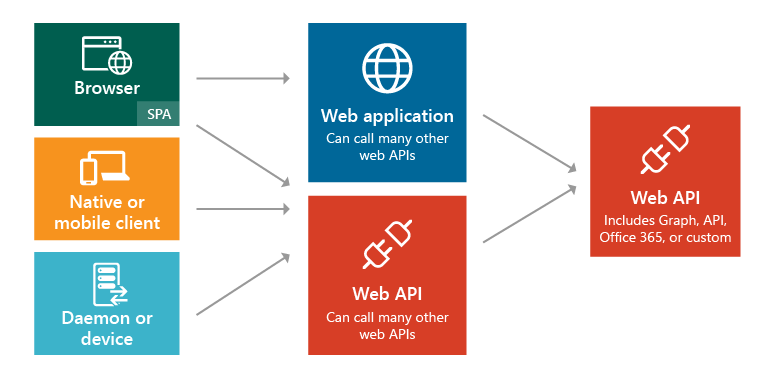
\includegraphics[width=\textwidth]{application_types}
    \caption{Типы приложений и сценарии}\label{fig:application_types}
\end{figure}

В каждом из этих сценариев предоставленная функциональность должна быть защищена от несанкционированного использования. Как минимум, обычно требуется проверка подлинности пользователя или участника, выполняющего запрос ресурса. Эта проверка подлинности может использовать один из нескольких распространенных протоколов, таких как SAML2p, WS-подача или OpenID Connect Connect. Взаимодействие с API обычно использует протокол OAuth2 и его поддержку для маркеров безопасности. Отделение этих критических проблем безопасности и их реализация от самих приложений обеспечивает согласованность и повышает безопасность и удобство обслуживания. Аутсорсинг этих задач на выделенный продукт, такой как IdentityServer, позволяет каждому приложению решить эти проблемы самостоятельно.

IdentityServer – это OpenID Connect и OAuth 2.0 фреймворк с открытым исходным кодом. OAuth — открытый протокол авторизации, который позволяет предоставить третьей стороне ограниченный доступ к защищённым ресурсам пользователя без необходимости передавать ей (третьей стороне) логин и пароль~\cite{wiki_oauth}. Вторая версия протокола была разработана с целью устранить недостатки первой версии связанные с плохой масштабируемостью и нетривиальностью использования на клиентской стороне. OpenID Connect - третье поколение OpenID-технологии, которое представляет собой аутентификационную надстройку над протоколом авторизации OAuth 2.0. OpenID Connect позволяет интернет-ресурсам проверить личность пользователя на основе аутентификации, выполненной авторизационным сервером. Для работы используется RESTful API, описанный в спецификации. Также в OpenID Connect определены дополнительные механизмы для надёжного шифрования и цифровой подписи.

IdentityServer - это официально сертифицированная реализация OpenID Connect. Поддерживается возможность работы с внешними сервисами, такими как Azure Active Directory, Google, Facebook и т.д~\cite{wiki_idenityserver}. Это ограждает приложения от подробностей о том, как подключаться к этим сервисам. Многие аспекты IdentityServer можно настроить в соответствии с конкретными потребностями. Поскольку IdentityServer - это фреймворк, очень просто написать код для адаптации системы в соответствии со специфическими сценариями. 

Использование фреймворка позволяет перенести ответственность за фундаментальные функции безопасности на сервис выдачи токенов, что предотвращает дублирование данной логики внутри приложений и внутренних сервисов.


\subsection{Vue.js}

Для реализации UI в данном дипломном проекте используется JavaScript-фреймворк Vue.js.

Vue.js – фреймворк~\cite{wiki_vue} с открытым исходным кодом для создания пользовательских интерфейсов. Он легко интегрируется в проекты с использованием других JavaScript-библиотек. Может функционировать как веб-фреймворк для разработки одностраничных приложений в реактивном стиле.

На данный момент поддерживается создателем Эваном Ю и остальными активными членами основной команды из различных компаний, таких как Netlify, Netguru, Baidu, Livestorm.

У Vue.js есть собственная официальная достаточно богатая документация на многих языках, выложенная на vuejs.org, которая может послужить примером в объяснении проектирования и разработки в браузере. 

К преимуществам фреймворка можно отнести:
\begin{itemize}
    \item малый вес фреймворка, что значительно ускоряет время загрузки страниц;
    \item высокая скорость разработки;
    \item хорошая документация и активное сообщество разработчиков;
    \item реактивность при помощи привязывания данных.
\end{itemize}

Основные библиотеки и инструменты Vue.js:
\begin{itemize}
    \item vue-router — официальный маршрутизатор для Vue.js.
    \item vuex — Централизованное управление состоянием на основе Flux для Vue.js.
    \item vue-loader — загрузчик веб-пакетов, который позволяет писать компоненты Vue в формате, называемом однофайловыми компонентами (SFC/Vue Single-File Component).
    \item Vue Server Renderer — рендеринг на стороне сервера для Vue.js
    \item vue-cli — стандартный инструментарий для быстрой разработки на Vue.js [11, 12].
    \item Vue Router — официальная библиотека маршрутизации для Vue.js. Она глубоко интегрируется с Vue.js и позволяет легко создавать SPA-приложения.
\end{itemize}

Vue Router включает в себя следующие возможности:
\begin{itemize}
    \item Вложенные маршруты/представления.
    \item Модульная конфигурация маршрутизатора.
    \item Доступ к параметрам маршрута, query, wildcards.
    \item Анимация переходов представлений на основе Vue.js.
    \item Удобный контроль навигации.
    \item Автоматическое проставление активного CSS класса для ссылок.
    \item Режимы работы HTML5 history или хэш, с автопереключением в IE9.
    \item Настраиваемое поведение прокрутки страницы.
\end{itemize}

Vue CLI — полноценная система для быстрой разработки на Vue.js, предоставляющая:
\begin{itemize}
    \item Интерактивное создание проекта через @vue/cli.
    \item Быстрое прототипирование через @vue/cli + @vue/cli-service-global без конфигурации.
    \item Большую коллекцию официальных плагинов, интегрирующих лучшие инструменты экосистемы фронтенда.
    \item Полноценный графический пользовательский интерфейс для создания и управления проектами Vue.js.
\end{itemize}

Vue CLI стремится стать стандартным инструментарием для экосистемы Vue. Он обеспечивает бесперебойную работу различных инструментов сборки, устанавливает разумные значения по умолчанию, поэтому вы сможете сосредоточиться на разработке приложения, а не проводить дни за его настройкой. В то же время остаётся гибкость настройки конфигурации каждого инструмента без необходимости извлечения конфигурации в отдельный файл.

\bigskip
\textbf{SASS}

Sass (Syntactically Awesome Stylesheets) — модуль, включенный в Haml. Sass — это метаязык на основе CSS, предназначенный для увеличения уровня абстракции CSS-кода и упрощения файлов каскадных таблиц стилей.

Одна из ключевых особенностей Sass — вложенные правила, которые облегчают процесс создания и редактирования вложенных селекторов.

К примеру, для вложенных правил, которые выглядят следующим образом:

\lstinputlisting[language=CSS]{appendix/sass_first.scss}

Получим следующую трансляцию в CSS:

\lstinputlisting[language=CSS]{appendix/sass_first_to_css.css}

Таким образом, определены инструменты и технологии для разработки программного средства. Основным языком программирования выбран \csharp за его быстродействие и эффективность в разработке. Для системы надёжного обмена данными между сервисами используется брокер сообщений RabbitMQ, а также бесплатный фреймворк с открытым исходным кодом MassTransit. На основе ряда преимуществ базой данных выбрана MongoDB. Для реализации надёжной авторизации пользователей используется фреймворк с открытым исходным кодом IdentityServer. Для реализации UI в данном программном средстве выбран JavaScript-фреймворк Vue.js.
